%\chapter{Habitat use and point process models} \label{sec:Chap1}
\chapter{Statistical Models for Individual-based Processes} \label{Chap1}

\section{Ecological Dynamics and Individual-based Models} \label{sec:Chap1_IBMs}

Ecologists study a tremendous range of topics, including for example:
\begin{itemize}
  \item How do different mechanisms of genetic mutation contribute to evolutionary dynamics \cite{hoffmann_revisiting_2008}?

  \item Why do particular traits arise independently in unrelated taxa, and how does this depend upon the environment \cite{pyenson_ecological_2017}?

  \item Under current global emissions of climate-altering gases and aerosols, how will the abundance, distribution, and function of ecosystems change \cite{li_spatial_2019}? 

  \item What is the diversity of microbes in the human body, and how does this affect behavior and disease \cite{dunn_internal_2020}?
\end{itemize}
These different questions have resulted in different research communities using different sampling and analytical methods, and it can be intimidating to look for any unifying framework that can unite theoretical and applied ecologists.

Despite this complexity, we seek a unified treatment of ecological dynamics.  By ``treatment" we mean a computational and analytical machinery that allows us to describe the ecological variables of interest, make accurate predictions while measuring our uncertainty, and simultaneously infer the impact of multiple mechanisms.  To accomplish these various goals, we generally define two things in the following:
\begin{enumerate}
    \item \textit{Individuals}, which could be an an individual organism, gene, or population;
    
    \item \textit{Marks}, which are properties of each individual that can change over time. These marks can include location, body size, age, maturity or energetic status, or other traits that are relevant to explain ecological patterns.
\end{enumerate}
At it's lowest level, we therefore describe dynamics from a \myindex{Lagrangian viewpoint}, where we seek to track individuals and how their characteristics (i.e., marks) change over time.  However, the Lagrangian viewpoint often becomes cumbersome and computationally impractical when the number of individuals increases.  In these cases, we then switch to describing dynamics using an \myindex{Eulerian viewpoint}. Instead of tracking individuals and marks, the Eulerian viewpoint tracks the number of individuals having a given mark within a given area.  For example, we might use the Lagrangian viewpoint to track the location \( S_j(t) \) of five individual \(j \in \{1,2,3,4,5\} \) individuals as a mark over time \( t \).  However, with 1000 individuals we might switch to the Eulerian viewpoint to instead track the number \( n_{s,t} \) of individuals within each area \(s\) at time \(t\).  In the following, we typically seek to introduce concepts using a Lagrangian viewpoint, and then transition to the Eulerian viewpoint when addressing that same concept for a large number of individuals.  

In particular, the Lagrangian viewpoint generally involves tracking the exact value of a given mark, e.g., location \( S_j(t) \), for individual \(j\) at any continuous time \(t\).  Changes in the value of each mark (it's ``dynamics") are then typically represented by some differential equation, e.g., where the location of animal \(S_j(t) \) might change as it moves in the direction of preferred habitats, or the size \( W_j(t) \) changes as it grows. In some special cases, it might be possible to calculate dynamics exactly, e.g., by solving the  differential equation analytically.  In practice, however, an ecologist will often specify dynamics for which there is no known exact solution, so dynamics must be approximated.  In other cases, an ecologist might want to explore different specifications for dynamics that involve different types of analytical solution, and may not want to learn different strategies to solve each version.  This again leads us to seek a general approach to approximate the outcome of a specified ecological process.  Approximations can vary greatly from high to low quality, where poor-quality approximations will result in large errors relative to a hypothetical exact solution.  In the following, we generally seek to approximate individual-based dynamics using \myindex{discretization}, which we define:
\begin{itemize}
    \item As methods that divide continuous space and/or time into a set of discrete and non-overlapping intervals (for time) or areas (for space), thereby replacing continuous dynamics (using differential equations) with discrete dynamics (using difference equations and linear algebra); 

    \item Where these methods are defined such that we can increase the resolution (i.e., the number of intervals and/or cells), and doing so will cause the approximation to be arbitrarily precise.
\end{itemize}
By emphasizing discretization, we hope to allow ecologists to balance their needs for accuracy (resulting from a high-resolution discretization), model flexibility (not being restricted to dynamics that can be solved analytically), and computational speed (resulting from initial exploration using low-resolution discretization).  

Ecologists generally recognize that ``nothing in biology makes sense except in the light of evolution" \cite{dobzhansky_genetics_1982,dobzhansky_nothing_1973}. From this we might take a few demographic principles that are true (with appropriate context) across all of ecology:
\begin{enumerate}
  \item All taxa must be composed of individual organisms that start their life with some assortment of traits;

  \item Similarly, all taxa are composed of individual organisms that produce new individuals, where these produced individuals (``children") have some similarity by descent to those individuals produced them (their ``parents"), whether by sexual or asexual production;

  \item Finally, all organisms will eventually die (such that the frequency of different traits can change without the total population size increasing infinitely).
\end{enumerate}
Beyond this (nonexhaustive) list of consequences of evolution, ecology is generally constrained by physical and thermodynamic constraints, e.g.:
\begin{enumerate}
  \item New individuals are typically smaller than the organisms that propagate them, and therefore will typically grow in size during life;

  \item Organisms cannot teleport through space, but must instead be transported continuously to move;

  \item Organisms must maintain some minimal metabolism to live, and death is irreversible (i.e., each organism will be born and die only once).
\end{enumerate}  
These demographic, evolutionary and thermodynamic principles imply that we can track the ``timeline" for each individual organism from the time of its birth to death, and also track the value of different ``marks", and thereby record the basic information about the individuals that make up a taxon. These principles also suggest a basic role for several marks, i.e., taxon \(c\), location \( s(t) \), time of birth \(t_{birth}\), time of death \(t_{death}\), age \( a(t) \), size \( w(t) \), and so on.  Continuous marks (such as location) can typically take any value from a specified continuous domain, while categorical marks (such as the species for a given individual) will take one of a specified set of levels.  Constructing machinery in this way is familiar to many ecologists as an \myindex{individual-based model} (IBM) or \textit{agent-based model}, and the performance of an IBM can be evaluated by determining whether a small set of individual rules or behaviors can reproduce system-level properties \cite{grimm_individual-based_2005}.   

\begin{table}
  \caption[Categorization of spatial data for ecological analyses]{Categorizing spatial data for ecological analyses by what type of spatial reference system is required to store it, based upon \cite{rowe_spatial_2022}.}
\begin{center}
\begin{tabularx}{\textwidth}{ | X m{2.5 in} m{1.5 in} | } 
  \hline
  Data category & Ecological example & Spatial object \\ 
  \hline

  Point data & Location for an individual & Point referenced data \\ & & \\ 
  
  Areal data & Count arising from visual sampling in a defined area & Areal referenced data  \\ & & \\ 
  
  Individual attributes & Size measurement for an individual & Attribute of an individual \\ & & \\

  Flow & Radar measurement of birds passing over a weather station & Directed graph data \\ & & \\

  Trajectory & A sequence of measurements of an animal's location over time & Sequence of points \\

  \hline
\end{tabularx}
  \label{tab:Chap1_ecological_data}
\end{center}
\end{table}

We also note that ecologists will often have different types of data, which arise from different ways of measuring ecological processes.  Here, we classify these based on how the data must be stored in a database, and arrive at five types of data:  point, areal, individual measurements, flow, and trajectory data (Table \ref{tab:Chap1_ecological_data}).  Different ecological systems will be relatively easy or hard to sample using these different categories.  For example, it is now feasible to directly measure animal foraging and energy expenditures using animals tags, such that data on individual habitat use and energy budgets is increasingly available for birds, mammals, and other animals \cite{curry_wildlife_2014}.  By contrast, measuring the movement of individual plants during their dispersal stage (i.e., pollen) or small insects remains difficult, and therefore point and areal data might be easier to collect than trajectories for these stages and taxa.  However, we seek a framework that can visualize and analyze all five categories of ecological data.  Given this context, we proceed by introducing two examples of IBM, and use these examples to demonstrate that we can often simplify these individual dynamics to define a computationally efficient statistical model.  

\section{Time-to-event Model for Individual Timelines}\label{sec:Chap1_time_to_event}

We first illustrate individual-based models by simulating the ``timeline" for each individual, which we define as the time of birth \(B_i\) and death \(D_i\) for each individual \(i\)\footnote{See https://github.com/james-thorson/Spatio-temporal-models-for-ecologists/Chap\_1 for code associated with this chapter.}.  We specify a constant birth rate, with \(r=0.2\) individuals born per year. This constant birth rate implies that the time elapsed from one birth \(B_i\) to the next \(B_{i+1}\) follows an exponential distribution:

\begin{equation}
  \Pr[B_{i+1} - B_{i} > \Delta_t] = e^{-r \Delta_t}    
\end{equation}
where we then record the birth time \(B_i\) for each individual occurring over 100 years.  

Similarly, we specify a Gompertz function for survival \cite{gompertz_xxiv_1825}. This Gompertz function is commonly fitted to survival-at-age tables, which list the proportion of individuals that are still alive at a given age. If we define the probability \(S(a)\) that an individual will survive to age \(a\), i.e., \(S(a) = \Pr[(D_i-B_i) > a]\) and define the derivative \(\frac{\text{d}}{\text{d}a} S(a) = -m(a) S(a)\) then \(m(a)\) is the mortality rate.  The Gompertz function specifies the mortality rate as: 

\begin{equation}
  m(a) = b e^{ka}    
\end{equation}
where \(b\) is the initial mortality rate when \(a=0\), and \(k\) defines an exponential increase or decrease in mortality rate with age.  The corresponding probability of surviving to a given age is then \cite{wilson_analysis_1994}:

\begin{equation}
  S(a) = e^{\frac{b}{k} (1-e^{ka})}    
\end{equation}
For illustration purposes in the following, we specify a low initial mortality rate \(b=0.001 \,  \mathrm{yr}^{-1}\), where the mortality rate accelerates exponentially at a rate of \(k=0.1 \, \mathrm{yr}^{-1}\).  To simulate the time elapsing between birth and death, however, we must convert the Gompertz survival function to the distribution of ages upon death (termed the ``lifetime density function").  In the terminology of a survival analysis, the Gompertz survival function  is converted to a lifetime cumulative distribution function \(F(a) = 1-S(a)\), and the derivative \(f(a)\) of the lifetime cumulative distribution \(F(a)\) is then the lifetime density function (Eq. \ref{eq:Chap1_f}):

\begin{equation} \label{eq:Chap1_f}
  f(a) = \frac{\text{d}}{\text{d}a} F(a)    
\end{equation}
In this example, we calculate the derivative symbolically using the function \colorbox{backcolour}{D} in R, and the function \colorbox{backcolour}{lifetime\_density} outputs this derivative (Code \ref{code:Chap1-R-symbolic-derivative}). We then use \myindex{rejection sampling} as explained in Appendix \ref{sec:rejection_sampling} to simulate values drawn from this lifetime density function \( f(a) \) (Code \ref{code:Chap1-R-rejection-sampling}).  

\lstset{style=Rcode}
\lstinputlisting[language=R, label=code:Chap1-R-symbolic-derivative, caption=R code applying symbolic derivative to calculate the lifetime density function., firstline=6, lastline=14, captionpos=t]{Chap_1/Gompertz_survival.R}

\lstset{style=Rcode}
\lstinputlisting[language=R, label=code:Chap1-R-rejection-sampling, caption=R code for rejection-sampling simulation of birth-death process., firstline=18, lastline=46, captionpos=t]{Chap_1/Gompertz_survival.R}

\begin{figure}[!ht]
    \caption[Individual-based model of births and deaths]{Gompertz survival function \(\Pr[(D_i-B_i) > a]\) (left panel black line) and resulting lifetime density function \(f(a)\) (left panel red line), along with one realization of individual timelines representing birth and death times over 100 simulated years (middle panel) and the total population size (right panel) resulting from this individual-based simulation.}
    \centering
    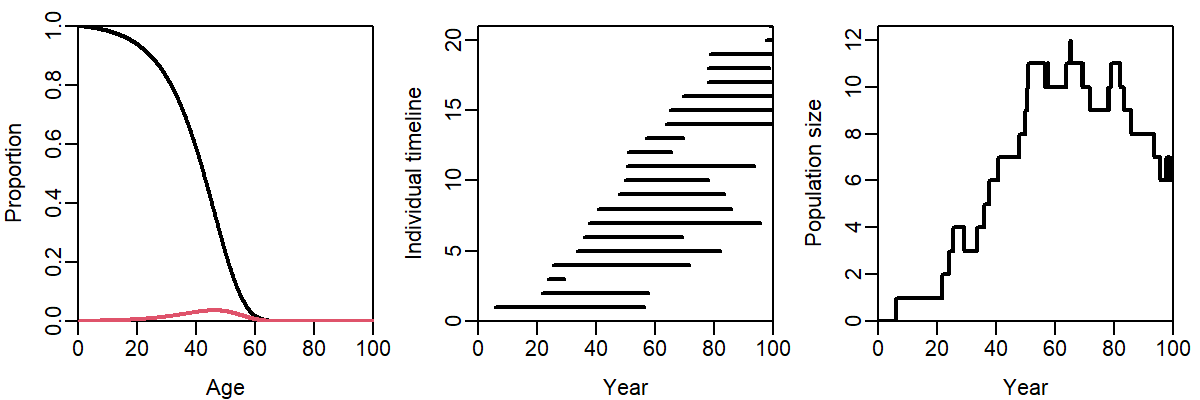
\includegraphics[width=5.5in]{Chap_1/Gompertz_survival.png}
    \label{fig:Chap1_gompertz}
\end{figure}

One simulation from this individual-based model (Fig. \ref{fig:Chap1_gompertz}) shows, e.g., that population size increased up until the maximum age of about 60 years, and then has a peak population size at around this time, arising due to stochastic variation in deaths occurring around that time. For now, we mainly note that this continuous process for births and death arising at one scale (i.e., for individuals) can then be coarsened to calculate stochastic variation in a function (i.e., population size), and that the function representing total population size \(n(t)\) will change by at most one individual over a sufficiently small step size (i.e., \(n(t)-1 \leq n(t+\delta) \leq n(t) + 1 \) as \(\delta\) approaches zero).  

\begin{table}
  \caption[Methods used for differentiation]{List of methods used throughout the textbook to calculate the slope of a line that is tangent to a specified function (called \myindex{differentiation}) \cite{baydin_automatic_2018}.}
\begin{center}
\begin{tabularx}{\textwidth}{ | X m{4in} | } 
  \hline
  Name & Description \\ 
  \hline

  Analytical & Memorizing several well-known transformations and applying them in sequence to a function \( f(x) \) to define a derivative function \( f'(x) \) that can later be evaluated to compute the derivative for any input \(x\) \\ & \\ 

  Numerical \newline(a.k.a. finite difference) & Evaluating a function (e.g., using a computer program) at several nearby locations, and approximating the derivative near those locations from the difference between these evaluated values; \\ & \\ 
  
  Automatic & In simplest form (called ``forward-mode AD"), writing a computer program that computes an output \( f(x) \) from inputs \(x\) using on a series of elementary operations, where the program evaluates these operations in sequence using supplied input values to calculate \(f(x)\) but also evaluates the derivative of these elementary operations (and automatically implements the chain rule) to compute \(f'(x)\), without directly storing an expression for \(f'(x)\) \cite{griewank_evaluating_2008,wengert_simple_1964}; \\ & \\

  Symbolic & Writing an expression to evaluate \( f(x) \), and passing this to a computer program that calculates an expression for \( f'(x) \). This expression might become very long as a result of the chain rule, but the expression can be written down and later evaluated to calculate \(f`(x\) for alternative inputs \(x\). \\
  
  \hline
\end{tabularx}
  \label{tab:Chap1_differentiation}
\end{center}
\end{table}

This example of sampling death times \(D_i\) from a negative derivative of the Gompertz survival function illustrates calculating a \textit{symbolic derivative}.  We will calculate derivates repeatedly throughout the book, alternatives to symbolic differentiation include numerical, analytic, and automatic differentiation (Table \ref{tab:Chap1_differentiation}).  Ecologists generally receive some background in analytical differentiation, but we suspect that many practicing ecologists find these methods intimidating such that methods requiring analytical differentiation will find limited use by applied ecologists.  As a result, we will generally emphasize numerical and automatic differentiation, which can efficiently implemented using software.  However, we will sometimes also present analytical derivatives if they are sufficiently simple to explain, and will use symbolic differentiation to check results from automatic differentiation.

We could instead approximate these individual dynamics using a model that tracks total population size \(n_t\) in a set of discrete times (e.g., using years \( t \in \{ 1,2,...,t_{max} \}\) and ages \( a \in \{01,2,..., a_{max}\}\)), and tracking the count of births \(b_{t,a}\) and deaths \(d_{t,a}\) for each age \(a\) in each year \(t\).   

\begin{equation}
\begin{gathered}
    b_{t,a=0} \sim \mathrm{Poisson}(\lambda = 0.2) \\
    d_{t,a} \sim \mathrm{Binomial}\left( n_{t,a}, \frac{F(a+1)-F(a)}{S(a)} \right) \\
    n_{t+1,a+1} = n_{t,a} + b_{t,a} - d_{t,a}
\end{gathered}
\end{equation}
where total abundance is calculated by summing across ages:

\begin{equation}
    n_t = \sum_{a=0}^{a_{max}} n_{t,a}    
\end{equation}
The Lagrangian viewpoint becomes infeasible when tracking millions of individuals, so it is convenient to understand both approaches to birth-death processes.

\section{Spatial Point Process for Habitat Utilization} \label{sec:Chap1_point_process}

Alternatively, we can specify an individual-based model (the Lagrangian viewpoint) as a spatial point process, involving marks for location \(s\) for each individual, and sum across space to calculate the total abundance within a specified spatial domain. To illustrate, we envision an immobile organism (i.e., a germinated plant) distributed along a gradient in elevation along the side of a mountain.  

\lstset{style=Rcode}
\lstinputlisting[language=R, label=code:Chap1-R-poisson-process, caption=R code simulating habitat utilization from an immobile organism arising from a point-process model., firstline=8, lastline=47, captionpos=t]{Chap_1/Poisson_point_process.R}

\begin{figure}[!ht]
    \caption[Individual-based model for habitat utilization]{Elevation (left), habitat quality (middle), and realized distribution for 500 individuals.}
    \centering
    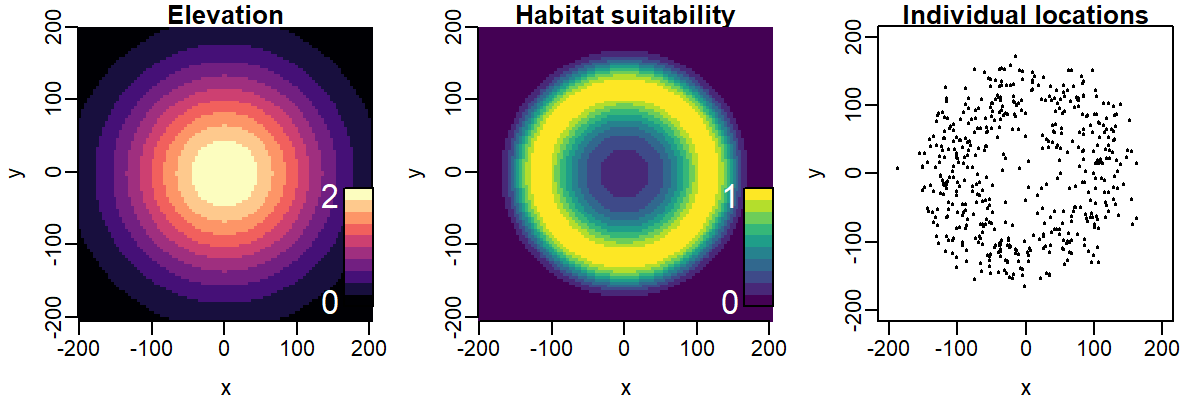
\includegraphics[width=5.5in]{Chap_1/Spatial distribution.png}
    \label{fig:Chap1_distribution}
\end{figure}

We specifically simulate elevation as a normal distribution with a peak of \(2\, \mathrm{km}\) and a standard deviation of \(100\, \mathrm{km}\).  We further envision that habitat suitability is greatest at \(1\, \mathrm{km}\) elevation, and declines as the squared log-ratio of elevation to this preferred value (Code \ref{code:Chap1-R-poisson-process}). We first illustrate the spatial distribution resulting from these assumptions (Fig. \ref{fig:Chap1_distribution}). Organisms are distributed independently in space (Fig. \ref{fig:Chap1_distribution}), such that the count of individuals \(N_A\) within a given area \(A\) follows a Poisson distribution:

\begin{equation}
\begin{gathered}
    N_A \sim\ \mathrm{Poisson}( \lambda_A ) \\
    \mathrm \lambda_A = \int_{s \in A} \lambda(s) ds
\end{gathered}
\end{equation}
hence the term \myindex{Poisson point process} for the resulting distribution of animal locations.  

We next discretize this Poisson point process by dividing the spatial domain into square grid cells, and treating abundance in each grid cell as if it follows a Poisson distribution.  This is an approximation, because we will use the elevation at the center of each grid cell as representing density for the entire cell.  However, this approximation can become arbitrarily precise as grid cells become smaller, so it qualifies as a ``discretization method" (recalling definition from Section \ref{sec:Chap1_IBMs}).  We then fit a generalized linear model to abundance \(N_i\) in each grid cell \(A_i\) for simulated organisms.  

\section{Generalized Linear Models} \label{sec:Chap1_GLM}

A \myindex{generalized linear model} (GLM) involves five components:

\begin{enumerate}
    \item A response variable \(y_i\) that we seek to explain and/or predict for each sample \(i\);
    \item A set of covariates \( \mathbf{x}_i\) that we use to explain the response variable, where covariates are specified as data and their values represent information associated with that sample;
    \item A vector of coefficients \( \mathbf{\beta} \) that we estimate from the model.  The product of coefficients and covariates is called the ``linear predictor" \( p_i = \mathbf{x}_i \mathbf{\beta} \);
    \item A \myindex{link function} \(g\), where the inverse-link function transforms the linear predictor into the mean of the responses such that \(g(\mu) = p_i\);
    \item A probability distribution \(f\) for responses given the inverse-link transformed linear predictor, \(g^{-1}(\mathbf{x}_i \mathbf{\beta})\), where additional ``measurement" parameters might be used to define this distribution.
\end{enumerate}

In the preceding example, we specify a log-linked Poisson distribution, where the log-density depends on log-elevation.  We specifically envision a circumstance where log-densities are highest at some intermediate elevation, and this is easy to specify using a quadratic function (i.e., including log-elevation and log-elevation squared as covariates):

\begin{equation}
\begin{gathered}
N_i \sim\ \mathrm{Poisson}( \lambda_i ) \\
\mathrm{log}(\lambda_i) = \beta_0 + \beta_1 \mathrm{log}(E_i) + \beta_2 \mathrm{log}(E_i)^2
\end{gathered}
\end{equation}
To demonstrate this point, we bin the area into 50 km by 50 km grid cells (Fig. \ref{fig:Chap1_gridded}), calculate the total abundance in each cell, and fit that with a log-linked Poisson GLM.  To do so, we use the R function glm (Code \ref{code:Chap1-R-GLM}); while fast, this approach does not give any particular insight into the mechanics of how the estimated value of parameters is identified, or how standard errors are calculated.

\lstset{style=Rcode}
\lstinputlisting[language=R, label=code:Chap1-R-GLM, caption=R code fitting GLM to point process., firstline=67, lastline=86, captionpos=t]{Chap_1/Poisson_point_process.R}

\begin{figure}[!ht]
    \caption[Gridded density of simulated above-ground-biomass]{A grid overlayed on the spatial domain, showing the location of individuals as well as the gridded value of above-ground-biomass, generated by counting the number of individuals in a given grid cell.}
    \centering
    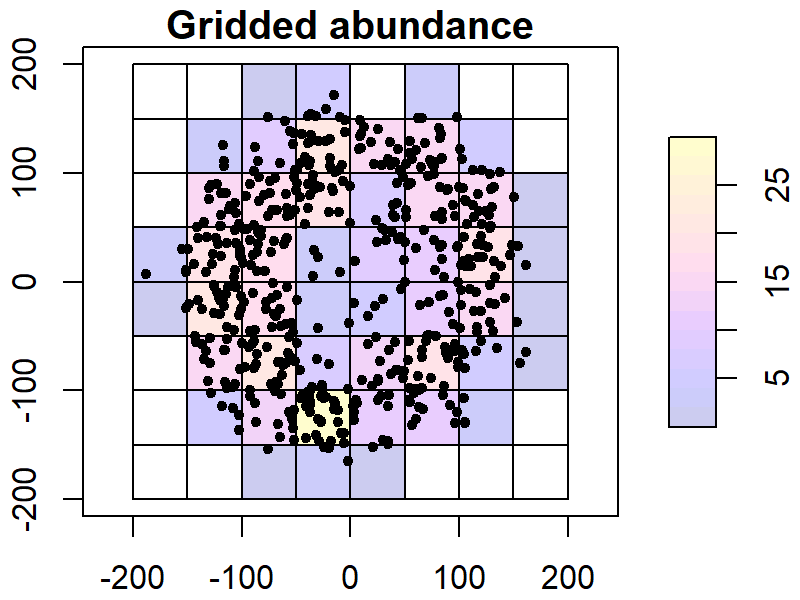
\includegraphics[width=3in]{Chap_1/gridded_density_res50.png}
    \label{fig:Chap1_gridded}
\end{figure}

\begin{table} 
  \caption[Estimated effect of elevation in gridded density in simulation experiment]{Estimated quadratic effect of elevation on simulated density of above-ground-biomass including estimated values, standard errors, T-value, and associated probability that the estimate differs from zero.}
  \catcode`"=9
  \centering
    \csvreader[
      tabular=|c|r|r|r|r|,
      respect all,
      table head=\hline \bfseries{} & \bfseries{Estimate} & \bfseries{Std. Error} & \bfseries{T-value} & \bfseries{Prob($>$0)} \\\hline,
      late after last line=\\\hline
    ]{Chap_1/glm_summary_res50.csv}{}{\csvlinetotablerow}
  \label{tab:Chap1_gridded}
\end{table} 

\section{Likelihood Estimation of Generalized Linear Models} \label{sec:Chap1_likelihood_GLM}

We next seek to replicate the GLM using a lower-level analysis that allows us to better understand the process by which parameters are estimated.  To do so, we take a detour into \myindex{maximum likelihood theory} \cite{fisher_mathematical_1922}.  

To illustrate maximum likelihood theory in a simple context, we envision that an analyst has some data \( y \) and can also specify a function \( y \sim\ f( \theta ) \) that is assumed to generate the data given unknown parameters \(\theta\).  We seek an estimator for \( \theta \) based on data \(y\), and one intuitive estimator is to pick the value of \( \theta \) that would then result in a high probability that the data take the values we observed \(y\).  This \myindex{maximum likelihood estimator} is (in a very loose sense) taking the hypothesized probability of data and using it in reverse to identify plausible values for parameters. The likelihood of data is often written as \( \Like( \theta; y ) \) and is then called the \myindex{likelihood function}. Maximum likelihood estimation involves identifying the value of parameters \( \theta \) that maximizes the likelihood function.  However, multiplying numbers often results in a computed likelihood that is larger than the largest digit that can be stored in computer software, or smaller than the smallest digit that can be stored (called \myindex{numerical overflow and underflow}, respectively).  We therefore instead compute the natural logarithm of the likelihood (the ``log-likelihood") such that numerical over and underflow is less likely to occur:  

\begin{equation}
    \hat{\theta} = \mathrm{argmax}_{\theta} \; \mathrm{log} \mathcal{L}( \theta; y )
\end{equation}

To understand the properties of this estimator \( \hat{\theta} \), we first remember that if two events \(A\) and \(B\) are independent, then the probability that these two events both occur is equal to the product of their individual probabilities, \( \Pr(A, B) = \Pr(A) \Pr(B) \).  The likelihood is itself a reinterpretation of the probability density \( p(Y \vert \theta) \), so it also shares this property:

\begin{equation}
    p(Y \vert \theta) = \prod_{i=1}^{n_i} p(Y_i \vert \theta)
\end{equation}
and replacing this with the log-likelihood:

\begin{equation}
    \mathrm{log} \mathcal{L}( \theta; y )  = \sum_{i=1}^{n_i} \mathrm{log} \mathcal{L}( \theta; y_i )
\end{equation}
This then shows that we can maximize the sum of log-likelihoods for each datum to calculate the total log-likelihood, as long as residuals are independent. 

We note that using \( \hat{\theta} \) as an estimator for unknown parameters \( \theta \) has several useful properties:

\begin{enumerate}
    \item \textit{Asymptotic consistency}:  if there's some value of parameters \( \theta \) such that function \( f( \theta) \) is a perfect description of the true data-generating process, then as data are added the maximum likelihood estimation \( \hat{\theta} \) will asymptotically approach the value \( \theta \).  

    \item \textit{Estimating uncertainty}:  we can estimate the uncertainty in parameters by calculating how quickly the log-likelihood declines as we change parameter values away from the maximum likelihood estimator \(\hat \theta\).  This involves measuring the curvature of the log-likelihood around estimator \( \hat{\theta} \), and one useful measurement is the matrix of 2nd derivatives for \( \log \mathcal{L}( \theta; y ) \)  with respect to \( \theta \) evaluated at its maximum value \(\hat \theta\), called the \myindex{Hessian matrix} \( \mathbf{H} \).  The matrix inverse of the Hessian, \( \mathbf{H}^{-1} \) approximates the variance of \( \hat{\theta} \) asymptotically (i.e., as the number of samples becomes large).
\end{enumerate}
In summary, maximum likelihood theory suggests that we can fit our Generalized Linear Model by calculating the loglikelihood for each datum, summing these, and then identifying the value of parameters \( \hat{\theta} \) that maximizes this loglikelihood, and this estimator will have good performance in terms of asymptotic consistency and uncertainty estimates.

\section{Estimation using Template Model Builder}

We next introduce \myindex{Template Model Builder} (TMB) \cite{kristensen_tmb_2016}.  TMB is an R-package that allows an analyst to write a ``template file" that calculates the loglikelihood; this template is written in C++ and therefore requires some basic familiarity with writing loops, indexing, etc.  Having written this template, however, TMB can then either calculate the likelihood, or use automatic differentiation to calculate a variety of gradients of the loglikelihood with respect to parameters. These values are passed back to R, and nonlinear minimizers in R can use the loglikelihood and its gradients to efficiently identify the value of \( \theta \) that maximizes the likelihood.  Calculating a ``cheap gradient" is key to using TMB to generalize almost all statistical operations that might interest us.  

\lstset{style=TMBcode}
\lstinputlisting[language=C++, label=code:Chap1-TMB-GLM, caption=TMB code defining the joint negative log-likelihood \colorbox{backblue}{jnll} for a generalized linear model using a Poisson distribution and log-link function., captionpos=t]{Chap_1/poisson_glm.cpp}

In the case of a GLM, we first write the template file that is interpreted by TMB (Code \ref{code:Chap1-TMB-GLM}).  We see that TMB requires several blocks of code:
\begin{enumerate}
    \item A header that defines the language, which will be identical in most files (lines 1--4 in Code \ref{code:Chap1-TMB-GLM});

    \item Functions (starting with syntax \colorbox{backblue}{DATA\_}) that define data passed from R (lines 5--7);
    
    \item Functions (starting with syntax \colorbox{backblue}{PARAMETER\_}) that define parameters passed from R (lines 9--12);
    
    \item Code defining variables that are used internally during TMB calculations (lines 14--17), where these are typically declared as scalars, matrices, arrays, etc., using a C++ type called \colorbox{backblue}{Type}. Declaring all variables as type \colorbox{backblue}{Type} then allows TMB to track either the value of variables, or their gradient with respect to parameters, depending upon which of these is useful at a given stage of parameter estimation;
    
    \item Code calculating the joint negative log-likelihood \colorbox{backblue}{jnll} based on data and parameters (line 21--31);
    
    \item Code that passes calculated values back to R, with the \colorbox{backblue}{jnll} in particular defining the joint negative log-likelihood.
\end{enumerate}
We will use TMB repeatedly, and will use a similar formatting of code blocks every time.

\lstset{style=Rcode}
\lstinputlisting[language=R, label=code:Chap1-R-GLM-in-TMB, caption=R code to compile and fit a GLM built in TMB., firstline=106, lastline=124, captionpos=t]{Chap_1/Poisson_point_process.R}

\begin{table}
  \caption[Estimated effect of elevation in gridded density using TMB]{Estimated quadratic effect of elevation on simulated density (see Table \ref{tab:Chap1_gridded} for details).}
  \catcode`"=9
  \centering
    \csvreader[
      tabular=|c|r|r|,
      table head=\hline \bfseries{} & \bfseries{Estimate} & \bfseries{Std Error} \\\hline,
      late after last line=\\\hline % horizontal line at the end of the table
    ]{Chap_1/tmb_summary_res50.csv}{}{\csvlinetotablerow}
  \label{tab:Chap1_TMB}
\end{table}

Finally, this code is compiled and linked as a \textit{dynamically linked library} in R (Code \ref{code:Chap1-R-GLM-in-TMB}).  This then allows for a cheap evaluation of the log-likelihood or its gradients. We can compare the output from this lower-level calculation with estimates using function \colorbox{backcolour}{glm} to fit a generalized linear model  (Table \ref{tab:Chap1_TMB}). We see here that the parameters estimates and standard errors for \colorbox{backblue}{beta\_j} are identical to those using \colorbox{backcolour}{glm}.  We can also plot the estimate of density, and compare it with the known true value (Fig. \ref{fig:Chap1_estimated_density}).

\begin{figure}[!ht]
    \caption[Simulation and estimate of gridded above-ground density]{True density (top-left), sampled total size (top-right), estimated density (bottom-left), and a comparison of estimated vs. true density (bottom-right) for the GLM fitted using TMB.}
    \centering
    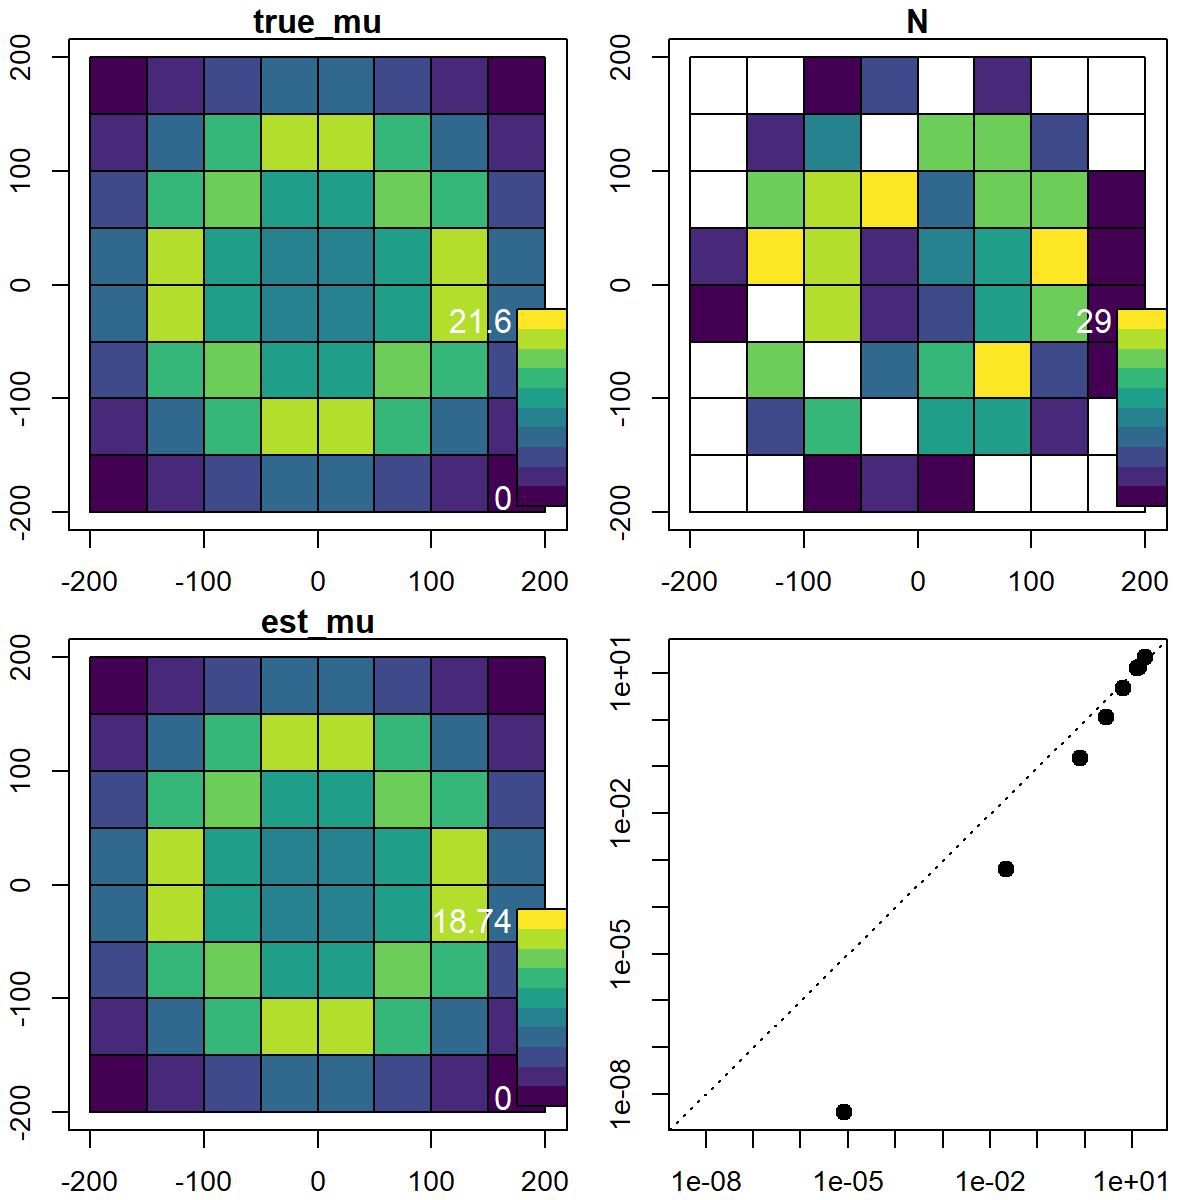
\includegraphics[width=5.5in]{Chap_1/estimated_density_res50.png}
    \label{fig:Chap1_estimated_density}
\end{figure}

\section{Evaluating Model Fit} \label{sec:Chap1_evaluating_model_fit}

Finally, ecologists will often want to compare model predictions with available data to determine whether there's evidence that the model is inconsistent with data.  Conceptually, one way to do this is to simulate data from the fitted model and then compare these simulated data with the real data to see if they are substantially different.  More formally, we can calculate \myindex{simulation residuals} to calculate the quantile for each datum.  This involves the following steps:
\begin{enumerate}
    \item For each observation, simulate new data conditional upon the maximum likelihood estimates of parameters \( \hat{\theta} \);

    \item Calculate the proportion of simulated values that are less than the real sample, and also the proportion that are less than or equal.
\end{enumerate}

\begin{figure}[!ht]
    \caption[Illustrating PIT residuals]{An illustration of how to calculate PIT residuals from a fitted model, which involves simulating from the fitted distribution for each datum and then calculating the quantile associated with each observation.  In the case of multiple simulations having the same value as an observation, the quantile is drawn from a uniform distribution within this range (see right-hand panel for example).}
    \centering
    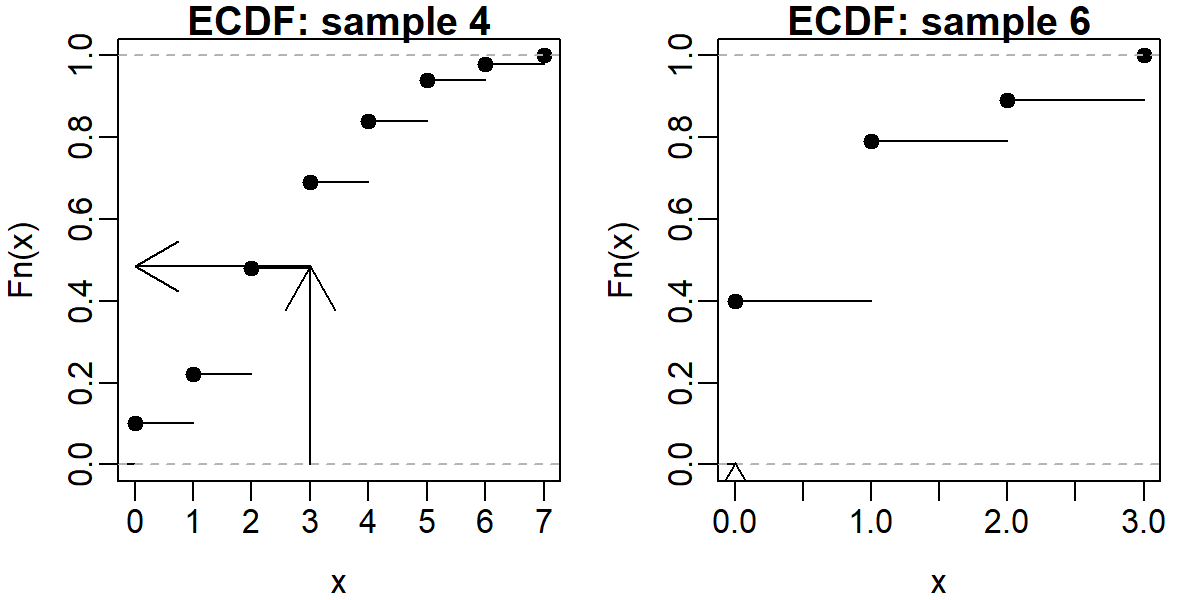
\includegraphics[width=5.5in]{Chap_1/simulation_residuals_res50.png}
    \label{fig:Chap1_PIT_example}
\end{figure}

\lstset{style=Rcode}
\lstinputlisting[language=R, label=code:Chap1-R-PIT-residuals, caption=R code for calculating and plotting the quantile residual diagnostic., firstline=153, lastline=170, captionpos=t]{Chap_1/Poisson_point_process.R}

For continuous-valued data, there is zero probability that any simulated sample will exactly match the observation, so the two values in Step-2 (i.e., the proportion less and the proportion less than or equal) will be identical, and the p-value can be calculated from either one.  Using the Poisson distribution (or other distributions for count data), however, the cumulative distribution for each sample follows a stair-step pattern because every simulated or real-world sample is a positive integer.  As a result, many samples might match a given observation and the two values in Step-2 would give different p-values.  For discrete-valued data, we therefore add another step:
\begin{enumerate}
    \item[3.] Randomly sample a p-value from a uniform distribution between these two values calculated in Step-2.
\end{enumerate}
This extra step is called the \index{probability integral transform}Probability Integral Transform (PIT) \cite{dunn_randomized_1996}, and it allows us to calculate a p-value for any mixture of discrete and continous data (see Fig. \ref{fig:Chap1_PIT_example}).  Step 1 involves simulating new data from the fitted model, which we enabled already using the function \colorbox{backblue}{SIMULATE} in the TMB code (line 28 and 34 of \ref{code:Chap1-TMB-GLM}).  We can then trigger this simulation by calling the function \colorbox{backcolour}{obj\$simulate()} in R.  Steps 2--3 are then done in R (Code \ref{code:Chap1-R-PIT-residuals}).

We can evaluate model fit by evaluating the quantile \(Q_i\) associated with each fitted sample \(y_i\). The quantiles for all samples are then compared with a uniform distribution; if the model is well specified, these quantiles will tend to follow a uniform distribution. We can therefore make a \myindex{quantile-quantile plot} and in some cases calculate a set of statistics that measure how different the simulation residuals are from a uniform distribution. In general, we will calculate these PIT residuals and summary statistics using the \colorbox{backcolour}{DHARMa} package \cite{hartig_dharma_2017} in R, where DHARMa then automatically takes care of calculations and plotting. In this case, the quantile-quantile plot shows no evidence of model misspecification (Fig. \ref{fig:Chap1_DHARMa_example}).  

\lstset{style=Rcode}
\lstinputlisting[language=R, caption=R code plotting quantile residuals using DHARMa., firstline=181, lastline=190, captionpos=t]{Chap_1/Poisson_point_process.R}

\begin{figure}[!ht]
    \caption[Example of quantile-quantile residuals]{Standard output from DHARMa, showing the quantile-quantile plot (left panel) with several goodness-of-fit tests listed (where a value $>$0.05 is non-significant (``n.s."), and also showing the rank-transformed predictions vs. residuals to see if there's a trend in either mean or 25/75th percentiles.}
    \centering
    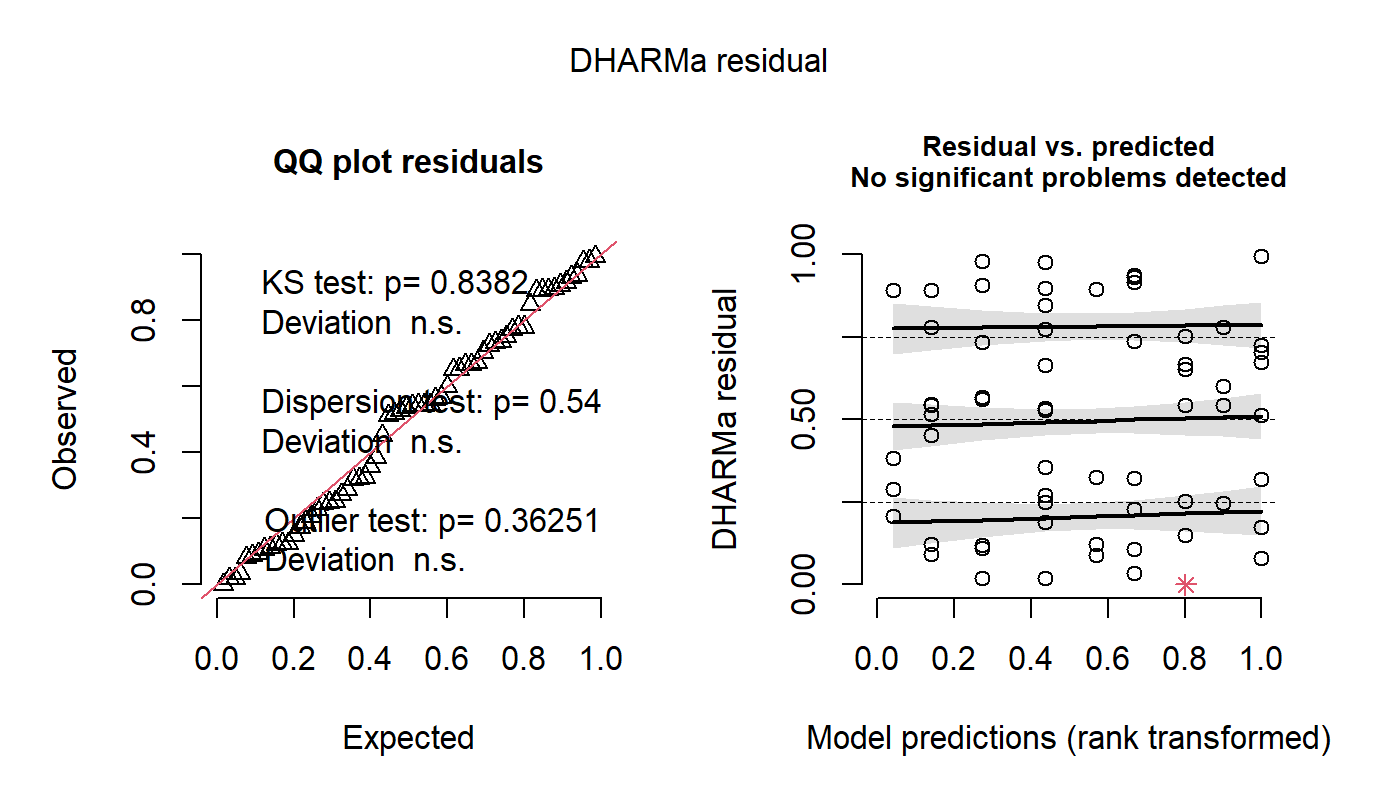
\includegraphics[width=5.5in]{Chap_1/DHARMa_residuals_res50.png}
    \label{fig:Chap1_DHARMa_example}
\end{figure}

We acknowledge that many ecologists are more familiar with Pearson residuals, which are calculated as the difference between a predicted and observed sample, divided by the estimated standard deviation for that sample, where these Pearson residuals are then compared with a normal distribution.  However, Pearson residuals have two major problems:

\begin{enumerate}
    \item \textit{Skewness}:  pearson residuals are typically compared with a normal distribution.  However, a model might specify a distribution (e.g., a lognormal) that has a higher probability of extreme events than the normal distribution predicts. In these cases, the Pearson residuals will seem to indicate a high number of outliers, even when those might be consistent with the distribution that was specified in the model;

    \item \textit{Misleading patterns}:  pearson residuals involve calculating the difference between predicted and observed values.  However, for count data, this difference is constrained to be an integer, such that Pearson residuals are sometimes constrained to some particular values and not others. This can result in visual artefacts when Parson residuals are plotted, and these then distract attention from other patterns that might actually identify model lack-of-fit.  
\end{enumerate}
Importantly, both of these problems are addressed by using PIT residuals.  

\lstset{style=Rcode} 
\lstinputlisting[language=R, label=code:Chap1-marginal-response, caption=R code visualizing an estimated covariate-response function and associated standard errors., firstline=202, lastline=216, captionpos=t]{Chap_1/Poisson_point_process.R}

\begin{figure}[!ht]
    \caption[Estimated response to elevation using coarse- or fine-scale discretizations]{A comparison of the estimated response curve (blue line) and its 95\% confidence interval (blue shaded area) against the true response curve (black line) using coarse 50 km \(\times\) 50 km grid cells (left-hand panel), or a finer-scale discretization, i.e., 10 km \(\times\) 10 km grid cells.}
    \centering
\begin{minipage}[a]{0.45\textwidth}
    $\vcenter{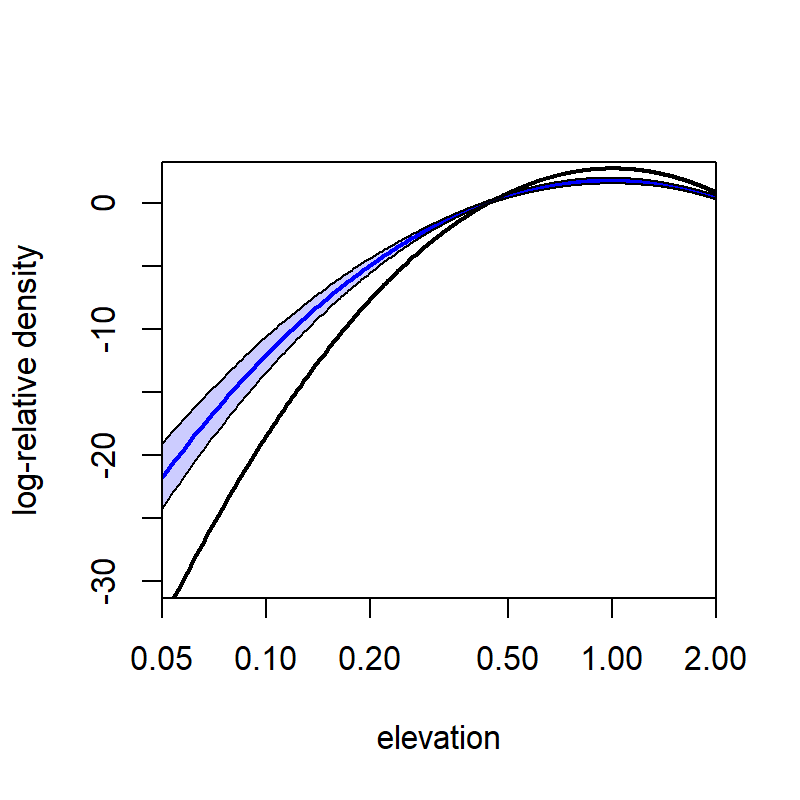
\includegraphics[width=2.75 in]{Chap_1/response_curve_res50.png}}$
\end{minipage}
\begin{minipage}[b]{0.45\textwidth}
    $\vcenter{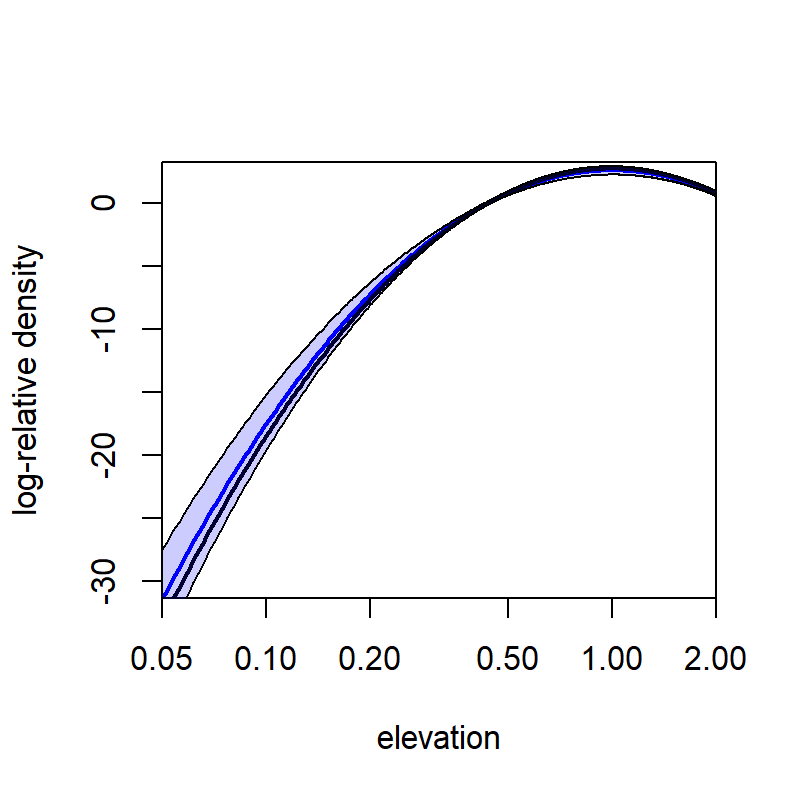
\includegraphics[width=2.75 in]{Chap_1/response_curve_res10.png}}$
\end{minipage}
    \label{fig:Chap1_response_curve}
\end{figure}

In additional to plotting residuals to identify any evidence of poor model fit, ecologists often use model selection to identify a parsimonious model from a set of candidate models. In general, ecologists can explore parsimony by conducting a crossvalidation experiment \cite{roberts_cross-validation_2017}, i.e.:
\begin{enumerate}
    \item Randomly divide the data into two bins, which are either fitted (\textit{in bag}) or withheld (\textit{out-of-bag}) from the model;

    \item Fit the model to the in-bag data;

    \item Use the fitted model to predict the out-of-bag data, either by computing their predictive log-likelihood or some other performance metric;

    \item Repeat these steps with different samples for in-bag and out-of-bag data, calculate average predictive performance across these samples, and select a model with best average predictive performance.
\end{enumerate}
However, conducting a crossvalidation experiment can be time-consuming for large models.  As a result, statisticians have developed approximations to the expected predictive performance that can be calculated from a fitted model without a crossvalidation experiment.  For example, ecologists often compute the Akaike Information Criterion (AIC) \cite{akaike_new_1974} and have been trained to report estimates arising from the model with the lowest AIC score \cite{burnham_model_2002}.  This model selection criterion favors models with good fit (i.e., a high log-likelihood) as well as fewer parameters, and can be viewed as one way to penalize covariate-response parameters towards zero \cite{hooten_guide_2015}.  Penalizing the number of model parameters arises because increasing the number of parameters also increases the expected difference in performance between fitted and new data (i.e., the log-likelihood for in-bag vs. out-of-bag data).  Alternative model-selection criteria can be adapted for the hierarchical models that we introduce in later chapters \cite{wood_smoothing_2016,vaida_conditional_2005}, although we generally do not emphasize model-selection in the following.  

Another important way to explore model fit is to visualize how predictions change for different covariate values.  Given that we are simulating data, we know the true covariate-response curve, and can evaluate model performance by comparing the true and estimated response curve relating log-density to elevation. To do so, we sample from the estimated covariance of fixed effects using a multivariate normal approximation.  We plot this estimated response against the known effect of elevation to evaluate how well the model did at reconstructing habitat preferences (Code \ref{code:Chap1-marginal-response}).  We observe, however, that the fitted response curve using this coarse-scale discretization (left-hand panel of Fig. \ref{fig:Chap1_response_curve}) does not perfectly match the known (simulated) effect of elevation.  We therefore refit using a finer discretization involving 10 km grid cells (instead of 50 km cells). This closer match (right-hand panel of Fig. \ref{fig:Chap1_response_curve}) provides visual confirmation that representing a Poisson point process as a Poisson GLM can in fact converge on the true data-generating process.  As noted in Section \ref{sec:Chap1_IBMs}, choosing a spatial scale for discretization requires balancing computational cost against other study goals.  We therefore recommend that analysts start with a coarse scale during early model development, increasing the resolution as the model becomes more refined, and both test and communicate the sensitivity of results to this choice. 

In later chapters, we will also automate the computation of these response curves using the \colorbox{backcolour}{marginaleffects} package \cite{arel-bundock_marginaleffects_2022}. To do this, we must define four functions for the model, and the \colorbox{backcolour}{marginaleffects} package subsequently calculates effects and standard errors (Code \ref{code:Chap1-marginaleffects-functions}).  This allows us to easily visualize the estimated responses to covariates (Fig. \ref{fig:Chap1_marginaleffects_curve}) using high-level plotting code (Code \ref{code:Chap1-marginaleffects-code}). 

\lstset{style=Rcode}
\lstinputlisting[language=R, label=code:Chap1-marginaleffects-functions, caption=R code defining functions used by the \colorbox{backcolour}{marginaleffects} package to visualize covariate-response curves., captionpos=t]{Shared_functions/marginaleffects.R} 

\begin{figure}[!ht]
    \caption[Partial effects generated using marginaleffects package]{Same as Fig. \ref{fig:Chap1_response_curve} but using the \colorbox{backcolour}{marginaleffects} package to generate response curves, and \colorbox{backcolour}{ggplot2} \cite{wickham_ggplot2_2016} to plot the response functions.}
    \centering
\begin{minipage}[a]{0.45\textwidth}
    $\vcenter{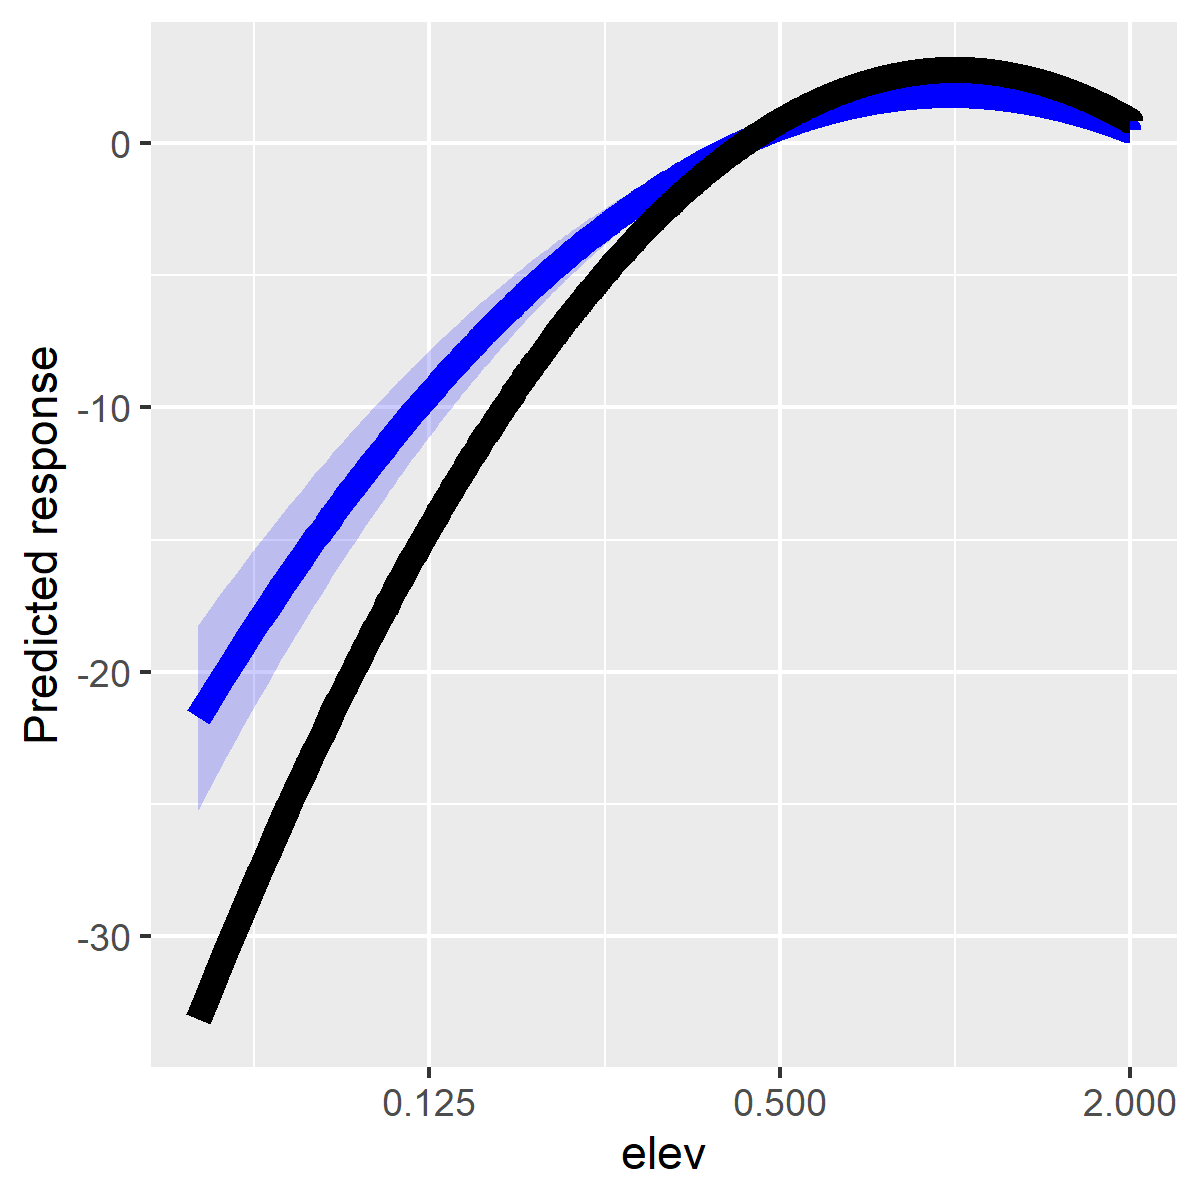
\includegraphics[width=2.75in]{Chap_1/marginaleffects_curve_res50.png}}$
\end{minipage}
\begin{minipage}[b]{0.45\textwidth}
    $\vcenter{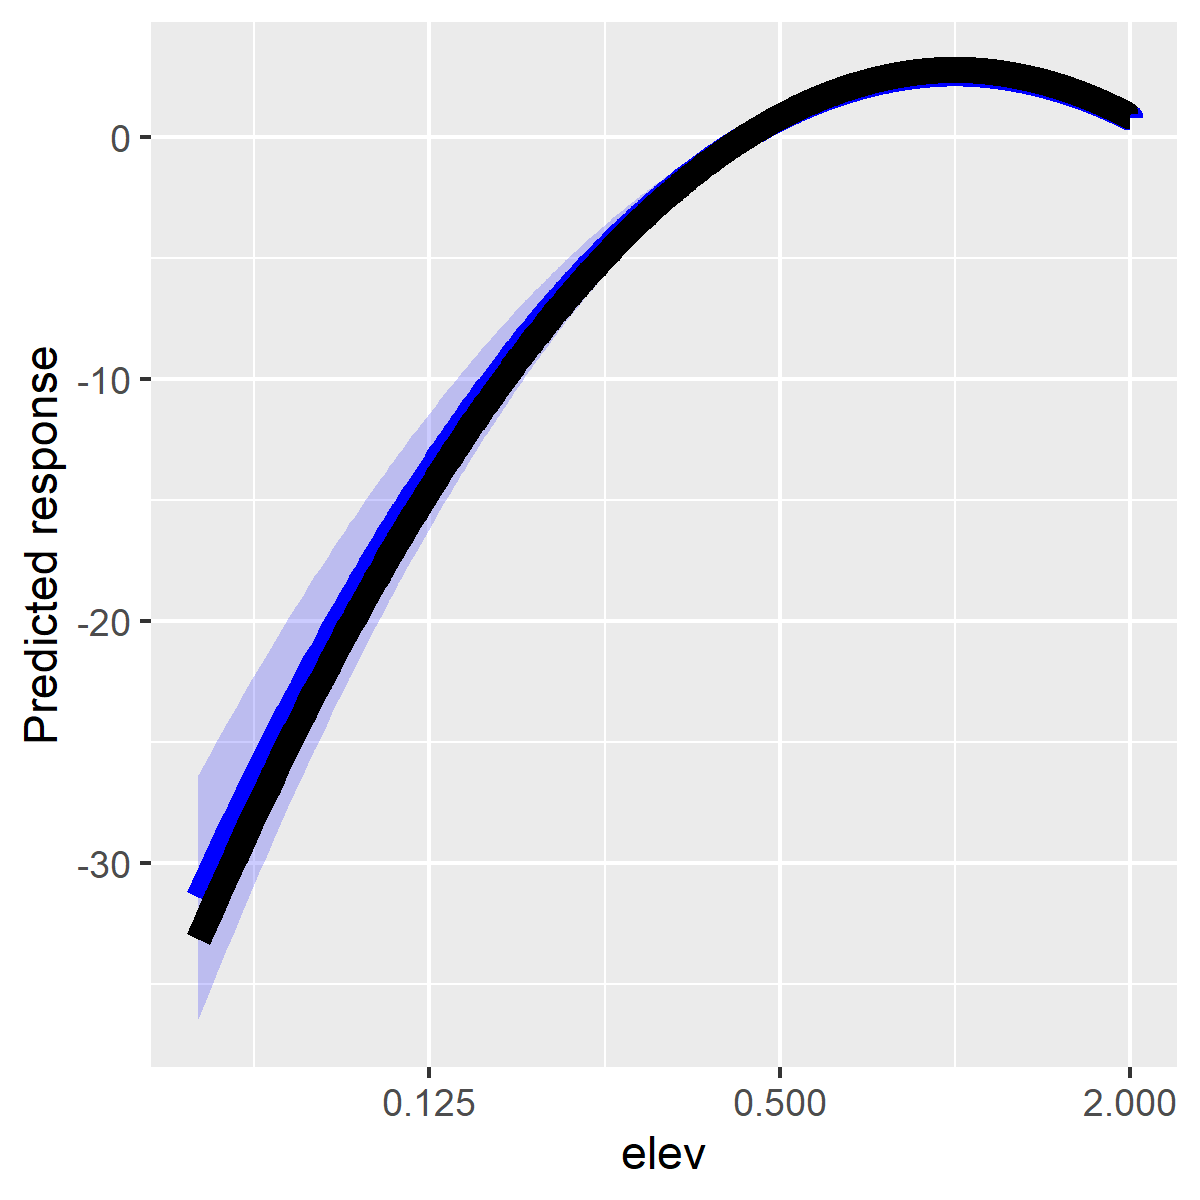
\includegraphics[width=2.75in]{Chap_1/marginaleffects_curve_res10.png}}$
\end{minipage}
    \label{fig:Chap1_marginaleffects_curve}
\end{figure}

\lstset{style=Rcode}
\lstinputlisting[language=R, label=code:Chap1-marginaleffects-code, firstline=232, lastline=257, caption=R code for using  the \colorbox{backcolour}{marginaleffects} package to produce covariate-response plots., captionpos=t]{Chap_1/Poisson_point_process.R} 

\section{Chapter Summary}

In summary, we have showed that:
\begin{enumerate}
    \item We can specify most ecological dynamics as an individual-based model by envisioning a set of ``individuals" where each individual has one or more ``marks".  These marks then represent an individual timeline (birth, death) and characteristics (size, location).  These marks may change over time, where, e.g., size changes due to growth and location changes due to movement.  In these cases, we are tracking changes using a ``Lagrangian" viewpoint.  However, this Lagrangian viewpoint becomes computationally infeasible as the number of individuals increase;

    \item We can generally approximate an individual-based viewpoint using an ``Eulerian" viewpoint, which tracks the number of individuals while dividing marks into bins.  For example, location (a continuous variable) can be binned into a series of grid-cells, or size (a continuous variable) can be divided into size bins \cite{merow_using_2014}.  In some cases, this approximation can become arbitrarily precise when binning data at a finer resolution, and we call this ``discretization" to distinguish it from the broader category of approximation methods;  

    \item An Eulerian viewpoint can in some cases be fitted as a Generalized Linear Model (GLM).  The GLM includes a linear predictor (calculated from covariates and estimated coefficients), a link function, and a specified distribution;

    \item A GLM can be fitted using maximum likelihood methods, which involves specifying a probability distribution for data, using this to calculate the log-likelihood of parameters given data, and maximizing this with respect to parameters; 

    \item The asymptotic performance of a maximum likelihood model can be understood using the central limit theory, and the model can be explored using PIT simulation residuals and by plotting marginal response curves using partial dependence plots. 
\end{enumerate}
We will use this statistical machinery throughout the remainder of the book.  We next explore cases when model residuals are correlated. The GLM assumed that residuals are independent (such that the log-likelihood can be summed across data), so correlated residuals then violate the assumptions involved in our analysis here. 

\section{Exercise}

Revisiting the time-to-event model for individual timelines (Section \ref{sec:Chap1_time_to_event}), what is the equilibrium abundance given the birth-rate and Gompertz survival parameters presented?  Please determine this in multiple ways and confirm the answer by comparing these.  Consider either simulating the sampling-based solution over a long time period and taking the average after equilibrium has been reached, or solving analytically (in the absence of stochasticity) by noting that population size is the product of birth rate and life expectancy, where the latter can be solved by integrating the survival function either analytically or using the \colorbox{backcolour}{integrate} function in R.  

% \end{minipage}
% \end{center}
